%!TEX root = ../Thesis.tex
We begin this chapter with the evaluation of the questionnaires and discuss the demographics and self-assessment of emotions felt by the subjects while watching the movies. We then take a look at how and which features were extracted from the Electrocardiogram (ECG) and Electrodermal activity (EDA) physiological data. Finally, we discuss how the extracted features were used to train a Random Forest machine learning model and a Long Term Short Memory (LSTM) \cite{lstm_hochreiter} neural network model for classification and prediction.

\section{Evaluation from the questionnaire}
As discussed in Section \ref{sec:procedure}, the subjects participating in the experiment were asked to fill in a questionnaire. The questionnaire constituted of two sections.
\begin{itemize}
    \item The first section comprised of demographic questions like age, gender, study program, language proficiency, and movie genre preferences.
    \item The second section of the questionnaire asked the subjects to self assess their emotions after each movie.
\end{itemize} 
The questionnaire was inspired by PANAS --- Positive and Negative Affect Schedule --- scale \cite{panas_crocker:1997} to quantify the emotions felt by the subjects while watching the movie. The questionnaire is attached in the appendix \ref{appendix_quest}. In the following section, we quantify the demographics and self-assessment of emotions felt by the subjects.
\subsection{Demographics}
\paragraph{Gender and age} The subjects participated in the study voluntarily. There was no prerequisite for participation in the study. A total of 72 subjects participated in the study of which 52 were male and 20 were female. The subjects were between 18-75 years old, with a mean age of 25.55 years and a standard deviation of 8.12 years. The age distribution is shown in figure \ref{fig:age_distribution}.

\begin{figure}
    \centering
    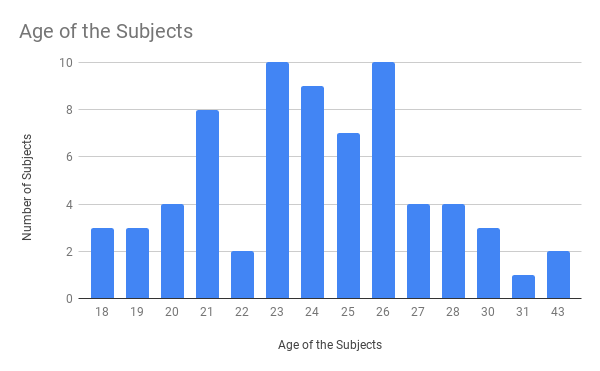
\includegraphics[width=140mm]{Figures/age_of_subjects.png}
    \caption{Age distribution of the subjects.}
    \label{fig:age_distribution}
\end{figure}

\paragraph{Language proficiency} The subjects were asked to rate their English and Spanish language proficiency between unfamiliar to native. The distribution of language proficiency is shown in figure \ref{fig:english_language} and figure \ref{fig:spanish_language}. As for the native languages of the subjects, 32 subjects spoke German, 19 subjects spoke Urdu, 10 subjects spoke Hindi, 2 subjects spoke Russian and one subject each indicated Chinese, Persian, Turkish, Vietnamese, English, Luxembourgian, Bengali, Hebrew, and Fula language.

\begin{figure}
    \centering
    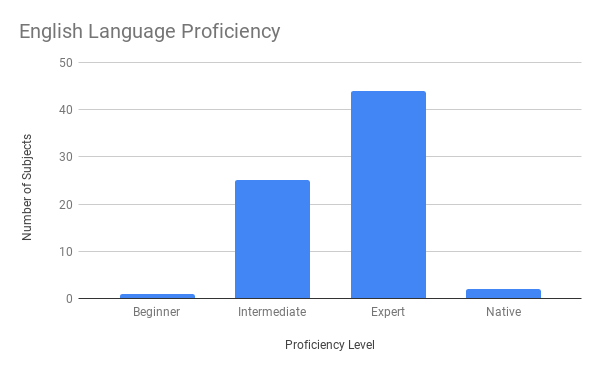
\includegraphics[width=140mm]{Figures/english_language_proficiency.png}
    \caption{English Language proficiency of the subjects.}
    \label{fig:english_language}
\end{figure}

\begin{figure}
    \centering
    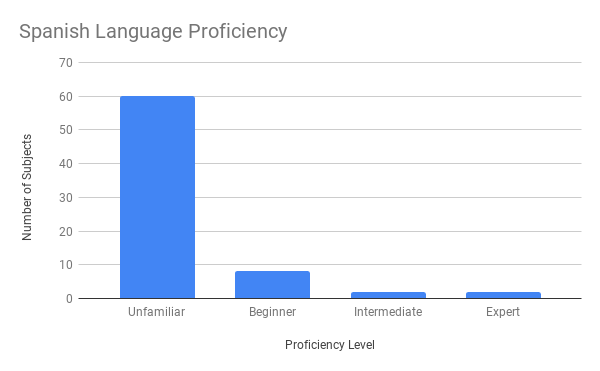
\includegraphics[width=140mm]{Figures/spanish_language_proficiency.png}
    \caption{Spanish language proficiency of the subjects.}
    \label{fig:spanish_language}
\end{figure}

\subsection{Self Assessment of Emotion}
The subjects were asked to assess how engaging the movie was for them and the emotions they felt while watching the movie. Figure \ref{fig:engagement_movies} gives an overview of ratings by the subjects as to how engaging the movies were. We see that except for a handful of instances, the subjects were moderately to extremely engaged in the movie. The subject's engagement in the movie is an important parameter. It shows that the ECG and the EDA data collected were indeed influenced by the subject watching the movie.
\paragraph{}
The emotions subject felt while watching the movie have been visualized in appendix 7.2. The emotions induced by different movies based on subjects assessment have been summarized in the table \ref{tab:emotions_self_assessment}. The table shows only the emotions that at least 50\% of subjects felt. We see that for every movie a different set of emotions were elicited. This is important as it would affect the ECG and EDA data differently as we discussed in chapter \ref{chapter:terminology}. 
\begin{center}
\resizebox{\textwidth}{!}{
\begin{tabular}{ |c|c|c| }
\hline
\textbf{Movie} & \textbf{Genre} & \textbf{Emotions} \\
\hline
\hline
3 Versos & Horror &  Amused, Aroused, Stressed, Fear \\
\hline
Alexia & Horror &  Amused, Disgust, Stressed, Fear \\
\hline
Go Bag & Action & Happy, Amused, Stressed \\
\hline
The Lie Detector & Comedy & Happy, Amused, Aroused, Neutral \\
\hline
The Last Three Minutes & Romance & Happy, Amused, Aroused, Neutral, Sad \\
\hline
I Miss You & Romance & Happy, Aroused, Sad \\
\hline
The Most Beautiful Thing & Romance & Happy, Amused, Aroused, Sad \\
\hline
\end{tabular}}
\captionof{table}{Short list of the movies selected for the study.}
\label{tab:emotions_self_assessment}

\end{center}

\begin{figure}
\centering
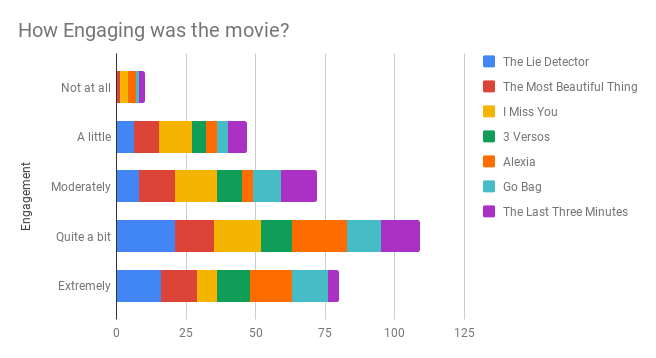
\includegraphics[width=140mm]{Figures/engagement.png}
\caption{Self assessment of engagement by subjects for the movies.}
\label{fig:engagement_movies}
\end{figure}

\subsection{Measure of discomfort due to electrodes.}
After the study session ended, the subjects were asked to rate whether they were distracted by the electrodes and if the electrodes caused any discomfort. This was to analyze if the presence of the electrodes may have caused some variation in the data compared to a less invasive wearable device. From the assessment made by the subjects, we found out that the presence of electrodes caused no to little discomfort amongst the majority of the subjects. The ratings of the users are presented in figure \ref{fig:discomfort}.

\begin{figure}
    \centering
    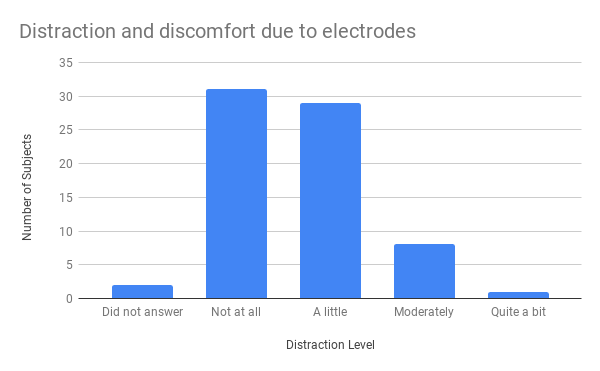
\includegraphics[width=140mm]{Figures/distraction_and_discomfort.png}
    \caption{Subject ratings of discomfort caused by electrodes.}
    \label{fig:discomfort}
\end{figure}

\subsection{Remarks}
There is an additional set of data that is considered in addition to the data from earlier mentioned 72 subjects. We took into consideration the data that we collected over the course of four months while we perfected the study procedure. We only selected the data whose signals had considerably low artifacts which could be removed by the techniques described in section \ref{sec:preprocessing}. Thus an additional physiological data set consisting of readings from 17 subjects were taken into consideration as well. The analysis includes ECG and EDA data of 89 subject in total.

\paragraph{}However, there is no demographic or emotional self-assessment questionnaire available for this data set. Verbal consent was taken from them for using their data pseudo-anonymously for this study. The dataset taken into account for this study is summarized in table \ref{tab:ecg_data_set} and table \ref{tab:eda_data_set} for ECG and EDA data respectively. The data collected before the questionnaire was introduced is termed 'old', and the data collected after the introduction of the questionnaire is termed 'new' in table \ref{tab:eda_data_set}. 


\begin{center}
\begin{tabular}{ |c|c|c|c| }
\hline
\textbf{Movie} & \textbf{Old} & \textbf{New} & \textbf{Total} \\
\hline
\hline
3 Versos & 11 & 33 & 44 \\
\hline
Alexia & 17 & 41 & 58 \\
\hline
Go Bag & 14 & 38 & 52 \\
\hline
The Lie Detector & 16 & 46 & 62 \\
\hline
The Last Three Minutes & 4 & 36 & 40 \\
\hline
I Miss You & 17 & 50 & 67 \\
\hline
The Most Beautiful Thing & 10 & 46 & 62 \\
\hline
\textbf{Total} & \textbf{89} & \textbf{290} & \textbf{379} \\
\hline
\end{tabular}
\captionof{table}{ECG Dataset.}
\label{tab:ecg_data_set}
\end{center}

\begin{center}
\begin{tabular}{ |c|c|c|c| }
\hline
 \textbf{Movie} & \textbf{Old} & \textbf{New} & \textbf{Total} \\
\hline
\hline
3 Versos & 10 & 32 & 42 \\
\hline
Alexia & 9 & 44 & 53 \\
\hline
Go Bag & 11 & 40 & 51 \\
\hline
The Lie Detector & 14 & 48 & 62 \\
\hline
The Last Three Minutes & 4 & 37 & 41 \\
\hline
I Miss You & 10 & 50 & 60 \\
\hline
The Most Beautiful Thing & 3 & 45 & 48 \\
\hline
\textbf{Total} & \textbf{61} & \textbf{296} & \textbf{357} \\
\hline
\end{tabular}
\captionof{table}{EDA Dataset.}
\label{tab:eda_data_set}
\end{center}

\section{Pre-processing of Data}
\label{sec:preprocessing}
\subsection{ECG}
\label{sec:ecg_feature_extraction}
The ECG data is obtained via BITalino's ECG sensor by measuring the voltage between the two electrodes with a low current applied between them. The third electrode acts as a voltage reference. The bandwidth of BITalino's ECG sensor is 0.5-40Hz; the accuracy of ECG readings is guaranteed in this range. The sampled value from BITalino's Analog Digital Converter (ADC) is a 10-bit signal value, \textbf{n}. We use a sampling frequency, \textbf{f$_{s}$} of 100Hz, 100 samples are recorded every second. The operating voltage, \textbf{V$_{CC}$}, of the ECG sensor, is 3.3V. The gain, \textbf{G$_{ECG}$} of the sensor is 1100. Thus, the raw data obtained from the BITalino device over the Bluetooth can be converted to ECG value in milli-volts using the transfer function described by the equation \ref{eq:ecg} \cite{ecg_datasheet}. The range of the ECG sensor is $\pm$1.5mV.

\begin{equation}
\label{eq:ecg}
    ECG(mV) = \frac{\big(\frac{ADC}{2^n} - \frac{1}{2})\times V_{cc}} {G_{ECG}}\times1000
\end{equation}

\subsubsection{Filtering} The lack of filter at the hardware level on the MCU \cite{noauthor_faq_nodate} of the BITalino resulted in some of the ECG signals obtained having artifacts. These artifacts were transient noise generated due to subject's movements during the recording. Thus there was further need for filtering the signals to eliminate the transient noise. We filtered the signal using bandpass FIR filter with cut-off frequency between 3-40Hz similar to the approach used by \citeauthor{canento_review_nodate} \cite{canento_review_nodate}. We then used Hamilton segmenter \cite{hamilton_open_2002} to detect the correct R-peaks. Figure \ref{fig:ecg_raw} and \ref{fig:ecg_filtered} visualizes the raw and filtered ECG signal respectively. The ECG signal is from one subject for 17 seconds while watching the movie \textit{3 versos}.

\begin{figure}
    \centering
    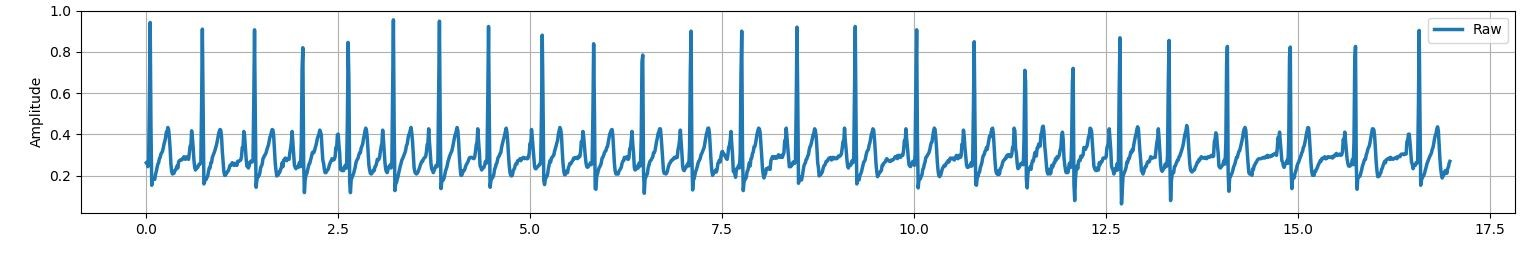
\includegraphics[width=140mm]{Figures/ecg_raw.jpg}
    \caption{Raw ECG Signal.}
    \label{fig:ecg_raw}
\end{figure}

\begin{figure}
    \centering
    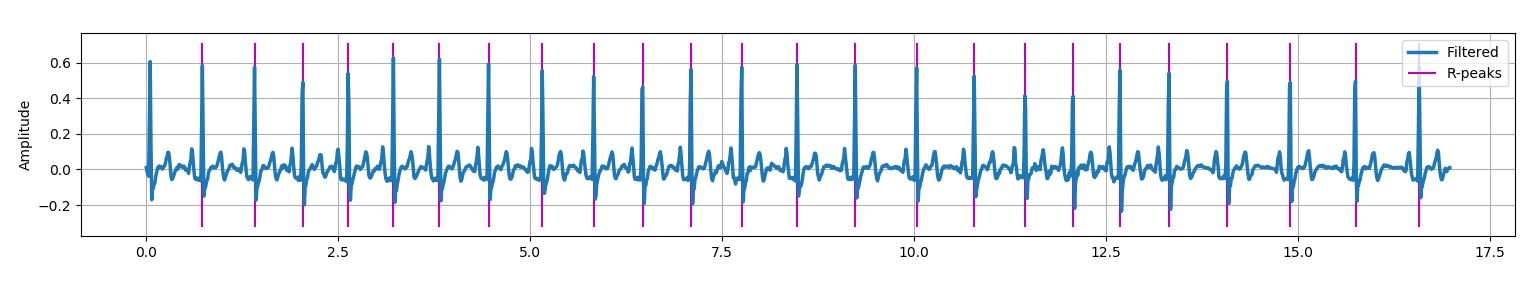
\includegraphics[width=140mm]{ecg_filtered.JPG}
    \caption{Filtered ECG Signal.}
    \label{fig:ecg_filtered}
\end{figure}



\subsubsection{Feature Extraction} 
\label{sec:ecg_fet_ext}
\paragraph{Heart Rate Variability (HRV)} R-R intervals (see section \ref{sec:rrinterval}) are obtained by measuring the distance between two consecutive R-R peaks. A statistical artifact detection was performed on the R-R intervals, to remove the R-R intervals that differed more than 25\% from the preceding R-R interval. Next, physiological artifact detection was performed to remove the R-R intervals that were less than 0.5 seconds or more than 1.3 seconds \cite{noauthor_normal_2018}. To put this into context of Heart Rate Variablity (HRV), the heart rates of more than 120 beats or less than 36 beats per minute were removed. The HRV is calculated from the R-R interval as we discussed in section \ref{sec:rrinterval}. Figure \ref{fig:ecg_hrv} visualizes the filtering of the ECG signal from one subject for 17 seconds segment of \textit{3 versos} movie.

\begin{figure}
    \centering
    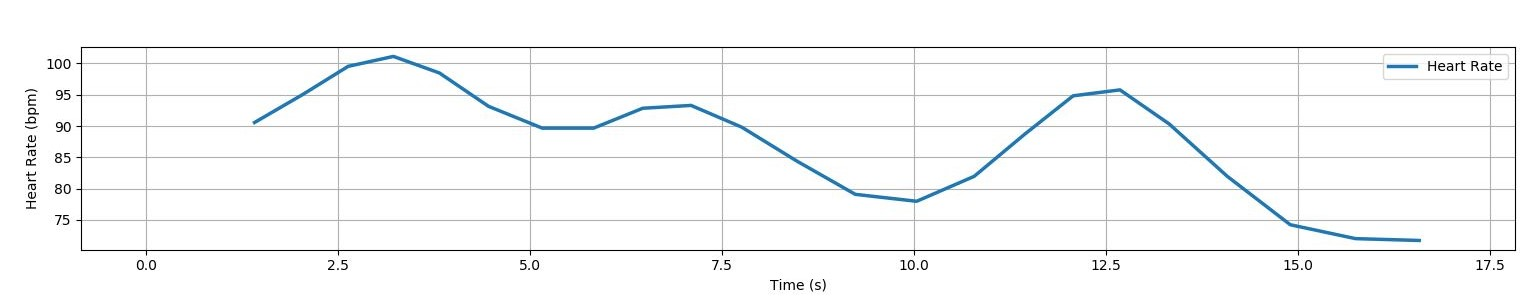
\includegraphics[width=140mm]{ecg_hrv.jpg}
    \caption{Heart Rate Variation (HRV) obtained from ECG Signal.}
    \label{fig:ecg_hrv}
\end{figure}

\paragraph{Frequency Components} The Low Frequency (LF) and High Frequency (HF) have been attributed to be influenced by the activity in Parasympathetic Nervous System (PNS) and Sympathetic Nervous System (SNS) \cite{noauthor_heart_1996} \cite{berntson_gary:1997}. We extracted the Low Frequency (LF) between 0.04-0.15Hz and the High Frequency (HF) between 0.15-0.40Hz. Furthermore, to see if there exists a correlation between other frequencies and PNS/SNS we also extracted Very Low Frequency (VLF) between 0.0033-0.04Hz and Very High Frequency (VHF) between 0.40-0.50Hz. We also computed the LF/HF ratio. the peak frequency of low frequency and high-frequency bands, LF/P and HF/P. In addition to that relative power of low frequency, LFn was computed with the equation \ref{eq:lfn} and relative power of high frequency, HFn with equation \ref{eq:hfn} \cite{shaffer_overview_2017}. 

\begin{equation}
\label{eq:lfn}
    LFn = \frac{LF}{\big(LF + HF)}
\end{equation}

\begin{equation}
\label{eq:hfn}
    HFn = \frac{HF}{\big(LF + HF)}
\end{equation}

\paragraph{Miscellaneous Features} In the paper published by \citeauthor{zhao_emotion_2016}, the authors found that there is a significant correlation between the emotions felt by the subjects and some of the frequency domain features discussed above, as well as time domain features and non-linear features \cite{zhao_emotion_2016}. Hence, we extracted the Standard Deviation of NN Intervals (sdNN), the Detrended fluctuation analysis (DFA), describing short-term fluctuations (DFA\_1) and long-term fluctuation (DFA\_1), the percentage of successive RR intervals that differ by more than 50ms (pNN50) and by more than 20ms (pNN20)  \cite{pend1995},  the Root Mean Square of Successive Differences (RMSSD), the Correlation-Dimension, and the Sample Entropy (SamEn) which measures the regularity and complexity of a time series. 

\subsection{EDA}
\label{sec:eda_feature_extraction}
The EDA is sensed by two AgCl electrodes. The EDA from the BITalino's EDA sensor is obtained by measuring the voltage between two electrodes across which a low current is applied. The bandwidth of BITalino's EDA sensor is in the range of 0-2.8Hz; accuracy is guaranteed in this range. The sampled value from BITalino's Analog Digital Converter \textbf{ADC} is a 10-bit signal value, \textbf{n}. Since we use a sampling frequency, \textbf{f$_{s}$} of 100Hz, 100 samples are recorded every second. The operating voltage, \textbf{V$_{CC}$}, of the EDA sensor, is 3.3V. Thus, the raw data obtained from the BITalino using the Bluetooth can be converted to EDA value in microSiemens using the transfer function described by the equation \ref{eq:eda}\footnote{The equation is adopted from the EDA sensor datasheet provided by the manufacturer \cite{eda_datasheet}. There is no explaination of why the value of 0.132 is used.}. The range of the EDA sensor is 0-25$\mu$S. 


\begin{equation}
\label{eq:eda}
    EDA(\mu S) = \frac{\big(\frac{ADC}{2^n}) \times V_{cc}}{0.132}
\end{equation}

\subsubsection{Filtering} The EDA values were obtained from the transfer function in equation \ref{eq:eda}. After visualizing the signal, we observed some artifacts in the EDA signal. This was evident as BITalino does not have any filter at the hardware level on the MCU \cite{noauthor_faq_nodate}. There was a transient noise in a few parts of the signal which occurred due to movements by the subjects during the experiments. In some signals, we also observed a static noise. This was probably because the manual denoising of the sensor as discussed in section \ref{sec:denoising}, did not effectively remove the static noise. We used the \textit{neurokit} \cite{noauthor_python_2019} package to filter the EDA signals. Butterworth Lowpass Filter from the package for was used to filter EDA signals. We set the cut-off frequency of 5Hz with order N=4 to decrease the noise. Figure \ref{fig:eda_filtering_} visualizes the filtering of the EDA signal from one subject while watching the movie, \textit{3 Versos}.

\begin{figure}
    \centering
    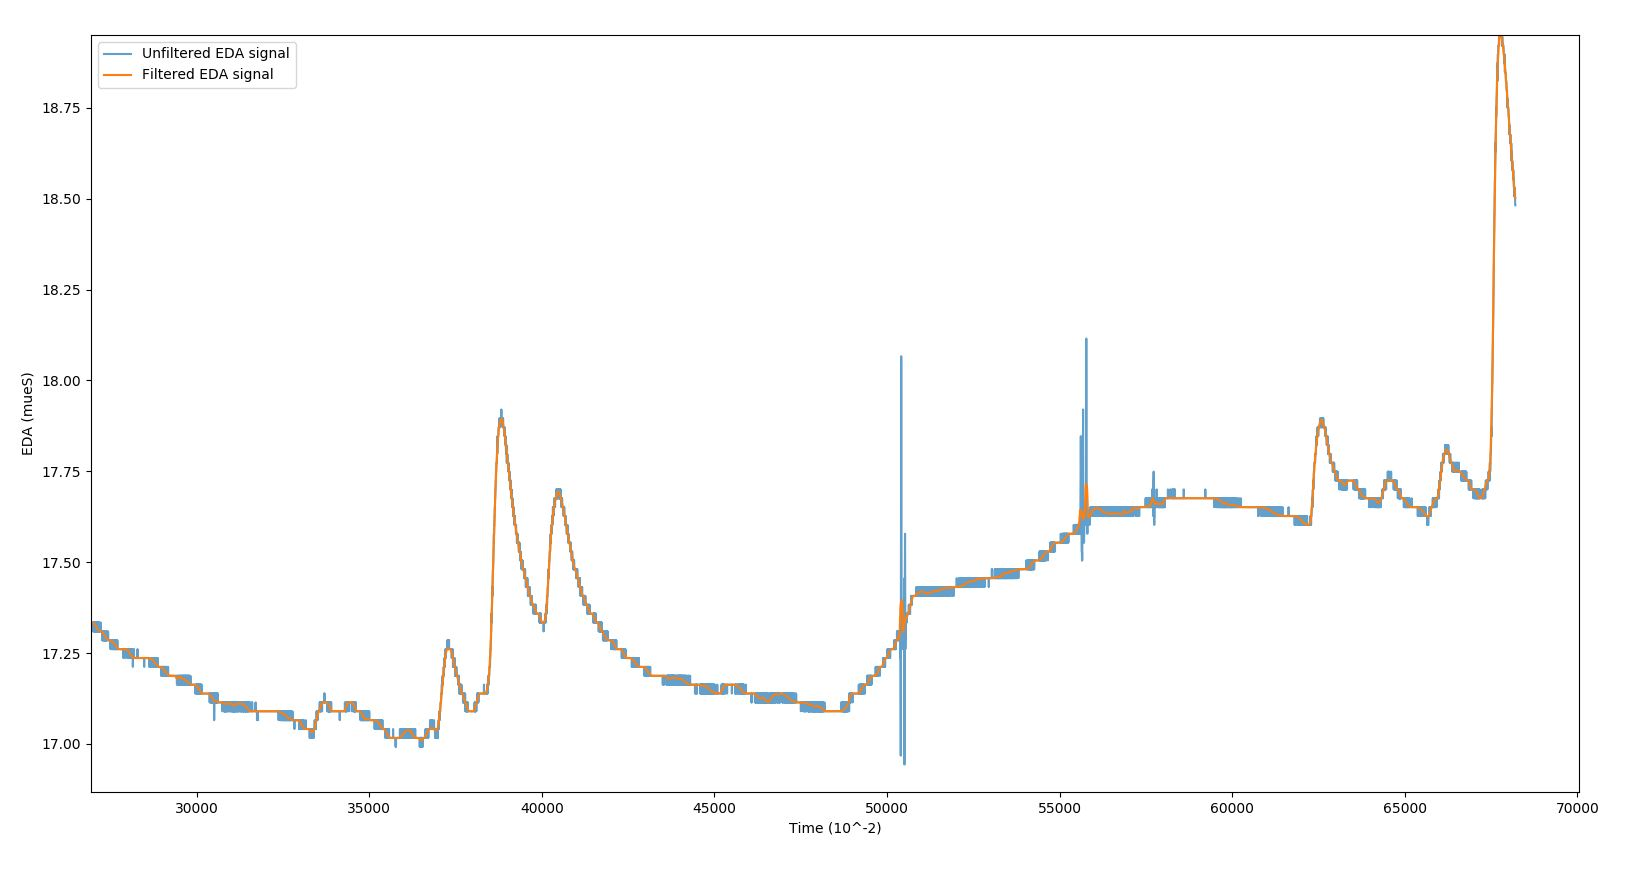
\includegraphics[width=140mm]{eda_filtering.JPG}
    \caption{Filtering of EDA Signal.}
    \label{fig:eda_filtering_}
\end{figure}

\subsection{Scaling}
\label{sec:eda_scaling}
We observed that the collected EDA data had a lot of variation between the subjects. Due to subjects physiology and state of mind during the study, some subjects had high EDA while others had low EDA. Also, some subjects had a larger variation in EDA over the period of the study than others. To normalize the EDA data, we applied scaling on the filtered data. The reason for applying to scale after filtering was to eliminate outliers and artifacts influencing of the EDA data. The scaling enhances the peaks for the EDA data with low variations. As discussed in section \ref{sec:eda_sensor}, the range of EDA sensor is between 0 to 25$\mu$S. So as to maintain that range for feature selection, we decided to scale the data between 0 to 25$\mu$S.

\paragraph{Remarks} Scaling of the ECG data was not required since we perform a feature extraction in the frequency domain.

\subsubsection{Feature Extraction}
\label{sec:eda_fet_ext}
\paragraph{Phasic Component} As we discussed in section \ref{sec:tonic_phasic_eda}, EDA can be described as the sum of three components: a slow changing tonic component, a fast changing phasic component, and an additive Gaussian noise due to measurement errors and artifacts. For our analysis, we required the phasic component, which is a fast-moving component influenced by an external stimulus. We thus used the cvxEDA algorithm proposed by \citeauthor{greco_cvxeda:_2016}\cite{greco_cvxeda:_2016} The algorithm is based on Bayesian statistics, mathematical convex optimization and sparsity. It has been shown to accurately decomposes the EDA signal into phasic and tonic components \cite{greco_cvxeda:_2016}. Figure \ref{fig:phasic_tonic_visualization} visualizes the filtered EDA signal, and the phasic and tonic component extracted from it. 

\begin{figure}
    \centering
    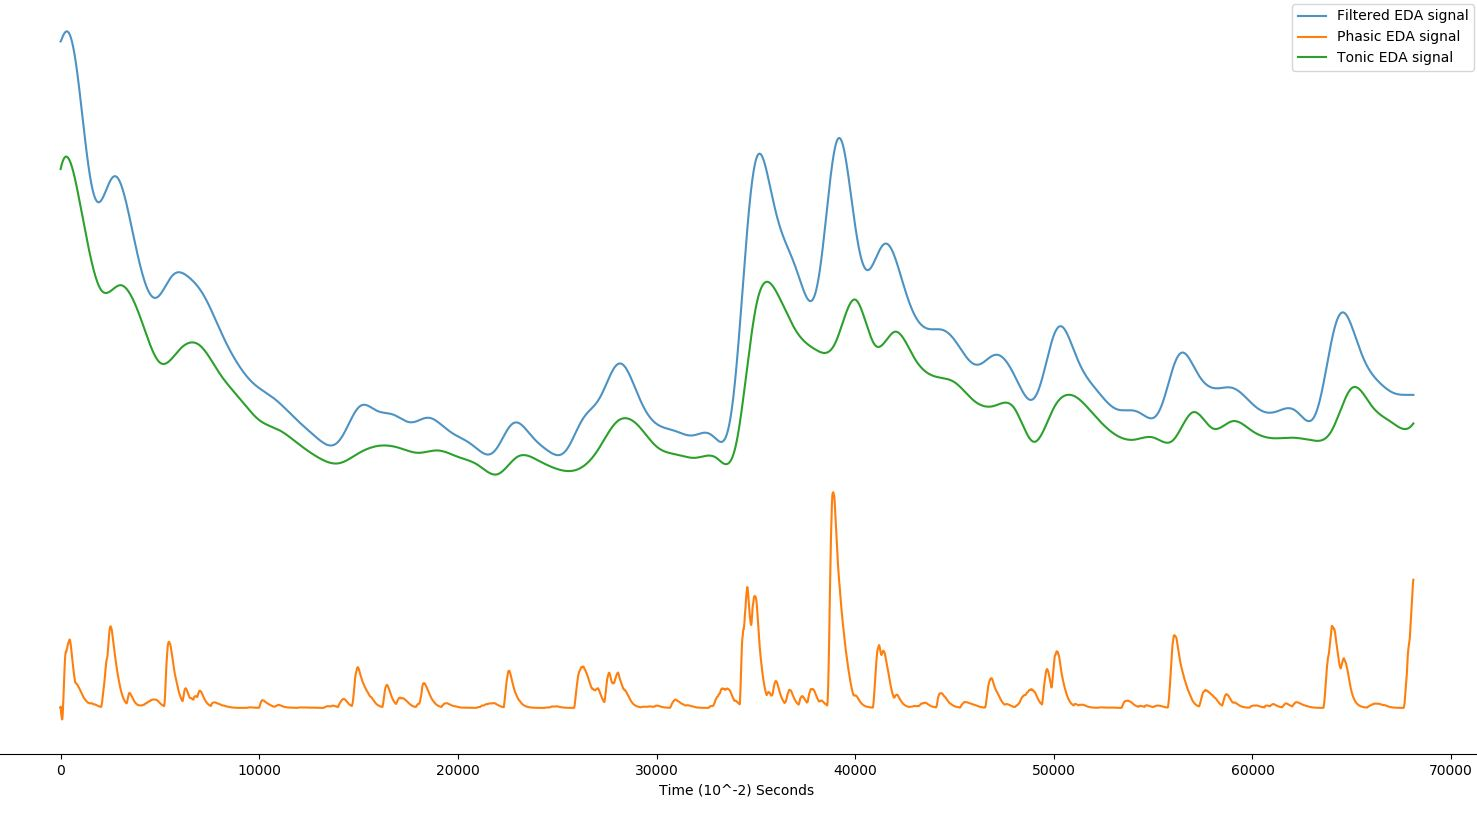
\includegraphics[width=140mm]{phasic_tonic_eda_visualization.JPG}
    \caption{Visualization of Phasic and Tonic EDA components.}
    \label{fig:phasic_tonic_visualization}
\end{figure}


\paragraph{EDA Onsets} As we have discussed in section \ref{sec:quantify_eda}, given the EDA in the time domain, the Onset can be defined as the time at which the external stimuli was induced on to the subject. This is resonated by a drastic increase in the EDA level and subsequently recovering after peaking in the time window of 3 to 5 seconds. This has been visualized in figure \ref{fig:eda_graph} in from chapter \ref{chapter:terminology}.

\paragraph{} We utilized the method proposed by \citeauthor{kim_emotion_2004} \cite{kim_emotion_2004}. The method detects the occurrence of EDA onset. In the first step, differentiation and subsequent convolution with the Bartlett window were applied on the filtered EDA signal by the authors. However, in our experiments, we did not downsample the signal for smoothing using the Bartlett window. We maintained the sample rate of 100Hz and window size of 100 since the result would be the same as the sampling rate of 20Hz and window size of 20. After convolution of the signal, the occurrence of the onset is detected by finding two consecutive zero-crossings, from negative to positive and positive to negative. The amplitude of the EDA is obtained by finding the maximum value between the two zero-crossing. The mean value of the amplitudes and the time point of the highest amplitude between the two zero-crossings is extracted as peak index and EDA onset respectively. We used the wrapper function provided by the \textit{neurokit} python package to extract the EDA features. The EDA Onsets extracted using this algorithm are visualized in figure \ref{fig:eda_onsets}.

\begin{figure}
    \centering
    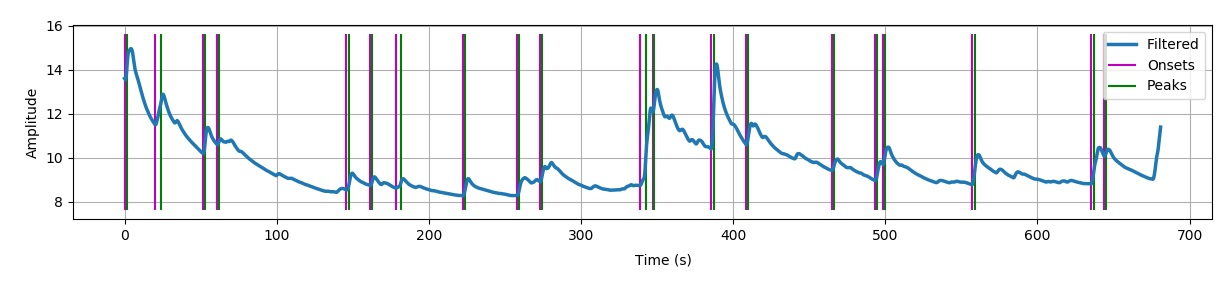
\includegraphics[width=140mm]{eda_onset.JPG}
    \caption{Visualization of EDA onsets.}
    \label{fig:eda_onsets}
\end{figure}

\section{Analysis and Results}
We extracted features for ECG and EDA as discussed in the previous section. The ECG features considered for our analysis are discrete values. The EDA features considered in our analysis is a time-series, phasic EDA. Classification of ECG features was done using a supervised machine learning algorithm, random forest. We chose to use random forest over Support Vector Machines (SVM) as it is better suited for non-linear dependencies. They also perform better for categorical/ numerical values. An added advantage is that random forest train faster and scale better as compared to SVM. The EDA features are time-series values. We utilized one of the Recurrent Neural Network (RNN) algorithms called Long Short Term Memory (LSTM) as they perform better than algorithms like ARIMA for classification of time-series data. Even though the training times are much longer for LSTMs, they are essentially a nonlinear time-series model, where nonlinearity is learned from data thus they are much more accurate that ARIMA. Thus they are better suited for our classification requirements. In this section we discuss our implementation, analysis and results of classification and prediction of our ECG and EDA data using random forest and LSTM respectively.

 \paragraph{Accuracy} In our analysis using random forest and LSTM we try find the accuracy of prediction of the our trained model. Given the features of ECG or EDA of subjects for the movies, the algorithm classifies the features based on the movies. The features from the test data are then used by the trained model to predict the movie they belong to. The accuracy is derived as the percentage of the movies that the model is able to predict correctly in the testing data. For example, given test data of ECG features of 10 subjects. If the model is able to predict 6 movies correctly then the accuracy of model is said to be 60\%. 

\subsection{ECG Analysis and Results}
\subsubsection{Approach}
\paragraph{Random Forest} Random forest \cite{breiman2001random} is a popular machine learning method based on decision trees. It is used for classification, regression or survival trees. In each split within the tree, the impurity reduction is maximized. This reduction is measured by the Gini index for classification, the sum of squares for regression and by the log-rank statistics or Harrell's C-index for survival outcomes \cite{wright_splitting_2019}. Random forest is part of the  ensemble methods. The ensemble methods combine the predictions of several base estimators built with a given learning algorithm to improve robustness over a single base estimator.

\paragraph{} In random forests each tree in an ensemble built from a sample from the training dataset. When splitting a node during construction the best split is a random subset of the features instead of the best split among the features. As a result, the bias of the forest increases as compared to the bias of the non-random trees. The variance of the random forests also decreases due to averaging. This compensates for the increase in the bias, thus yielding a better model.
\paragraph{} All the implementation of the algorithm were done using Python 3.6 on a 96 core machine with a clock speed of 2.7GHz and 512GB of RAM.

\subsubsection{Analysis}
\paragraph{Data Preparation}  We performed the filtering, scaling and feature extraction as discussed in the section \ref{sec:ecg_feature_extraction}. No further processing was done on the extracted features.

\paragraph{Implementation} We implemented a random forest classifier to classify the ECG features based on the movies. Several features were extracted, but not all of them are useful for our analysis. Hence, we wanted to understand which features are significant for the classification of the movies. Therefore, we ran a feature selection algorithm on top of the random forest. We used the recursive feature elimination and cross-validation (RFECV) \cite{sklearn_rfecv} selection algorithm to select the significant features.

\paragraph{} In our analysis, we selected the features based on the paper by \citeauthor{zhao_emotion_2016} \cite{zhao_emotion_2016} to classify emotions. We included some other features to see if we find any correlation between those features and the movies they associate to. These features were then fed into the RFECV. RFECV uses random forest algorithm to select the best features. Thus, we determine the subset of our selected features which are significant in increasing the accuracy of prediction.

\paragraph{} In all our evaluation, the ECG data for all the movies mentioned in table \ref{tab:shortlist_movies} were taken into consideration. The dataset was split as 90\% for training and 10\% for testing. Since there was a large variance between the samples of the dataset, we decided to run our implementation 10 times with a randomized split each time to avoid false-positive results. To put it in a nutshell, a different set of training and testing data was selected from the dataset for each evaluation. From a total of 379 data samples in the data set, 341 samples were used for training and 38 samples were used for testing.

\subsubsection{Results}
\label{sec:ecg_analysis_results}
\paragraph{Features} Here we took into consideration the pNN50, Standard Deviation of NN Intervals (sdNN), the LF/HF ratio, the Sample Entropy (SamEnt), the DFA$_{1}$ and the DFA$_{2}$ features extracted from the ECG dataset (see \ref{sec:ecg_fet_ext}). The results are summarized in the table \ref{tab:ecg_rf_results}. The 'True' notation means that the feature was selected in the training phase to determine the accuracy of the model and 'False' notation means that the feature was not selected. The overview of 10 evaluations shows that 7 times of 10, all the features were selected for the training of random forest and yielded an accuracy of 39\% on an average. That is out of every 10 predictions, the random forest algorithm was able to predict the movie correctly 4 times. We note that since 7 movies are under consideration, the probability of a movie being recognized by chance is about 14\%. As a side note, the test and training data was shuffled every time the model was being trained and tested. This is why we have some variations in the prediction accuracy shown in table \ref{tab:ecg_rf_results}. Thus, we conclude that there exists a correlation between the subject's ECG data and their viewing activity as discussed under our goal for the thesis in chapter \ref{chapter:motivation}. However, the results can be further improved. Our suggestions on improving the results are presented in section \ref{sec:future_work}. We also tested the other features that were extracted but not used. None of them yielded any significant improvements in our results.

\begin{center}
\resizebox{\textwidth}{!}{
\begin{tabular}{ |c|c|c|c|c|c|c|c| }
\hline
&\multicolumn{6}{c}{\textbf{Features of ECG}}& \\
    \cline{2-7}
\textbf{Evaluation} & \textbf{sdNN} & \textbf{pNN50} & \textbf{LF/HF} & \textbf{DFA$_{1}$} & \textbf{DFA$_{2}$} & \textbf{SamEnt} & \textbf{Prediction Accuracy} \\
\hline
\hline
1 & \textbf{True} & False & \textbf{True} & \textbf{True} & \textbf{True} & \textbf{True} & 31\% \\
\hline
2 & \textbf{True} & \textbf{True} & \textbf{True} & \textbf{True} & \textbf{True} & \textbf{True} & 38\% \\
\hline
3 & \textbf{True} & False & \textbf{True} & \textbf{True} & False & \textbf{True} & 24\% \\
\hline
4 & \textbf{True} & \textbf{True} & \textbf{True} & \textbf{True} & \textbf{True} & \textbf{True} & 46\% \\
\hline
5 & \textbf{True} & \textbf{True} & \textbf{True} & \textbf{True} & \textbf{True} & \textbf{True} & 37\% \\
\hline
6 & \textbf{True} & False & \textbf{True} & False & False & \textbf{True} & 35\% \\
\hline
7 & \textbf{True} & \textbf{True} & \textbf{True} & \textbf{True} & \textbf{True} & \textbf{True} & 43\% \\
\hline
8 & \textbf{True} & \textbf{True} & \textbf{True} & \textbf{True} & \textbf{True} & \textbf{True} & 37\% \\
\hline
9 & \textbf{True} & \textbf{True} & \textbf{True} & \textbf{True} & \textbf{True} & \textbf{True} & 35\% \\
\hline
10 & \textbf{True} & \textbf{True} & \textbf{True} & \textbf{True} & \textbf{True} & \textbf{True} & 36\% \\
\hline
\end{tabular}}
\captionof{table}{Analysis of results of LSTM model on physiological dataset on the movies.}
\label{tab:ecg_rf_results}
\end{center}

\subsection{EDA Analysis and Results}
\label{sec:eda_ana_results}
\subsubsection{Approach}
\paragraph{LSTM} Neural networks are a powerful tool for pattern classification based on deep learning techniques. LSTM is one of the powerful recurrent neural networks used for time-series classification and pattern recognition. In it's early day, the LSTM models used concept of self-circulation
to generate a path for long-term continuous flow of gradients. \cite{long_short_hochreiter}.  The important addition to the LSTM was to make the weight of self-looping were made context-sensitive rather than fixed. The weights of the self-loop are derived from the gated structure and the accumulated time scale can be dynamically changed. This helped to over come the problem of traditional recurring neural networks which used an excessive number of layers in time-series data. The correlations between time-series, long and short were handled by using a hidden layer as a memory unit in LSTM network. 

\begin{figure}
    \centering
    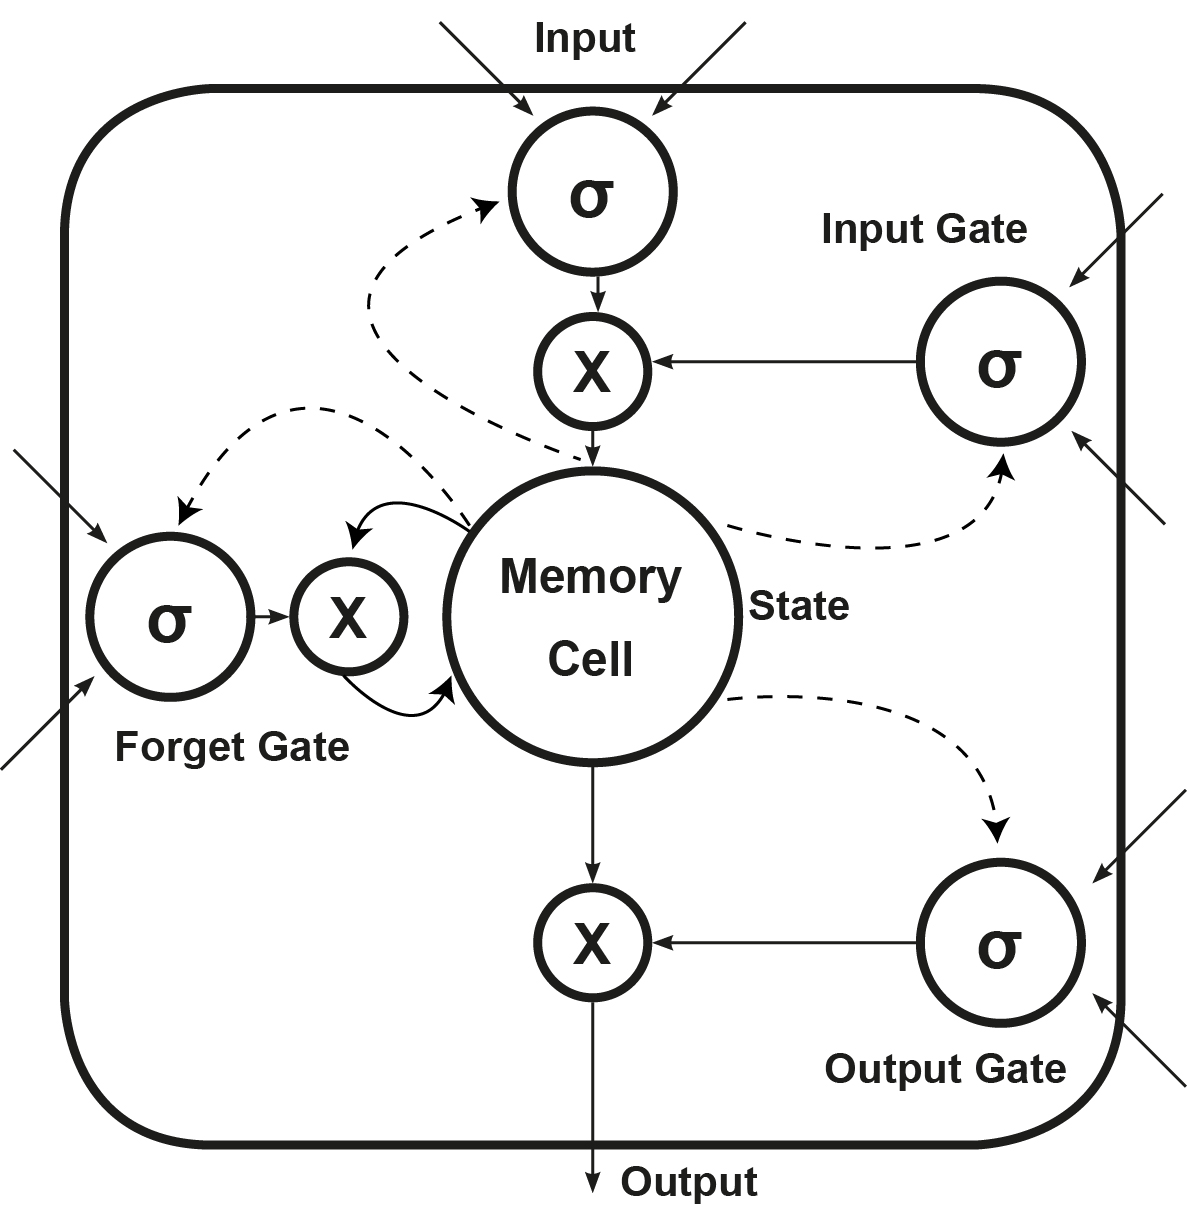
\includegraphics[width=140mm]{lstm.jpg}
    \caption{Structure of the LSTM \cite{liu_td-lstm:_2018}.}
    \label{fig:lstm_structure}
\end{figure}
\paragraph{LSTM Structure} The most widely used LSTM structure is visualized in figure \ref{fig:lstm_structure} \cite{liu_td-lstm:_2018}. In this model, the  \textit{input gate} controls if or not a value can be added to a \textit{memory cell}. The \textit{state} unit can be linearly self-looping, and its weight is controlled by a \textit{forget gate}. The \textit{output} of the cell is controlled by the \textit{output gate}. All gate units can perform a sigmoid nonlinear transformation, and the input unit can have any compression non-linearity. The LSTM network can be defined by the following series of the equation:

\begin{equation}
\label{eq:lstm_threshold}
    i_{t} = \sigma \small(W^iH + b^i)
\end{equation}
\begin{equation}
\label{eq:lstm_forget_gate}
    f_{t} = \sigma \small(W^fH + b^f)
\end{equation}
\begin{equation}
\label{eq:lstm_output_gate}
    o_{t} = \sigma \small(W^oH + b^o)
\end{equation}
\begin{equation}
\label{eq:lstm_new_state}
    c_{t} = tanh \small(W^cH + b^c)
\end{equation}
\begin{equation}
\label{eq:lstm_output}
    m_{t} = f_{t}\cdot m_{t-1} + i_{t}\cdot c_{t}
\end{equation}
\begin{equation}
\label{eq:lstm_6}
    h_{t} = tanh\small(o_{t}\cdot m_{t})
\end{equation}

In the equations a sigmoid transformation ($\sigma$) is performed on threshold values (\textit{i$_{t}$}), forget gate values (\textit{f$_{t}$}), and output gate values (\textit{o$_{t}$}). An activation function (\textit{tanh}) is computed on new states of the cell (\textit{c$_{t}$}) to avoid gradients from exploding. \textit{W$_{i}$}, \textit{W$_{f}$}, \textit{W$_{o}$}, and \textit{W$_{c}$} denote the respective weight matrices of threshold, forget gate, output gate, and new state. The offset terms are denoted by \textit{b$_{i}$}, \textit{b$_{f}$}, \textit{b$_{o}$}, and \textit{b$_{c}$}.  \textit{H} is the concatenation of the new input \textit{x$_{t}$} and the previous hidden vector \textit{h$_{t-1}$}. The final state of the cell \textit{m$_{t}$} is calculated by the sum of the dot product of the forget gate value and the final state of previous memory cell, and the threshold values and the new state values of the cell. The output of the memory unit is derived by calculating the dot product of the output gate values and the final state of current memory cell. An activation function (\textit{tanh}) is applied to the dot product. 

\paragraph{} In the following sections, we will discuss the two implementations of LSTM we did to analyze our data. To reiterate, we are trying to train the model to predict the movies based on the test data. We will describe the data prepared for the training, the hyperparameters and the implementation of LSTM, and the results.

\subsubsection{base-LSTM Model}
\label{sec:lstm_base_model}
\paragraph{Data Preparation}

We performed the filtering, scaling and feature extraction as discussed in section \ref{sec:eda_feature_extraction} to get the phasic EDA for all subjects and movies. We trained this model for the phasic EDA, with different combinations of hyperparameters and group sizes of movies. The phasic EDA feature was chosen for the training as it is derived from the EDA and reflects the response of the subject to external stimuli. This is based on the literature we discussed in section \ref{sec:tonic_phasic_eda}. Different parameters were chosen to fine tune our model. In our initial analysis of results, we found that the accuracy of the model was very high due to the fact that the different lengths of the movies were allowing our model to predict the correct movie easily. Thus, we then altered the data fed to our model. We considered the smallest length of the sample in the data under scrutiny for the group of the movies and pruned the beginning part of all other samples to match the sample with the smallest length. Since the smallest movie in our dataset is of only 120 seconds and the longest movie is of 823 seconds, it was important for us that analysis was performed properly on the available dataset. Second, with different group sizes, we wanted to understand if our model is scalable. Thus, we tested our model for a combination of two, three, four, five and six movie groups. 

\paragraph{Architecture} The base model comprises of a single hidden layer followed by a dropout layer intended to reduce overfitting of the model to the training data. Two dense fully connected layers are used to interpret the features extracted by the LSTM hidden layer followed by a softmax logistic regression layer. The dense layer employs rectified linear units (ReLUs) to compute the feature maps. A number of recurrent dense layers can be employed to improve the accuracy of the model. \citeauthor{karpathy_visualizing_2015} \cite{karpathy_visualizing_2015} showed that depth of at least two recurrent layers is beneficial when processing of sequential data. To be more time efficient, we limited our analysis to two recurrent dense layers as the increase in the number of layers would significantly increase the processing time. 

\paragraph{Hyperparameters} We used the Keras \cite{keras} package to do our analysis. In the LSTM layer, we used the default \textit{tanh} activation function as we discussed earlier this is to avoid gradients from exploding into very large values. After which we used a dropout layer with a value of 0.5 to reduce overfitting of our model. As discussed above we used rectified linear units (ReLU) as an activation function for the dense layer. We used the Adam gradient \cite{kingma_adam:_2014} for the gradient optimization algorithm and categorical cross entropy loss function as it is a multi-class classification problem. 

\paragraph{Model implementation and training} We ran the training data with different size grouping of the movies. The sampling rate of physiological data used in the dataset was maintained at the sampling rate of 100Hz. To be more time efficient, not all the combinations were tested. We randomly selected the movies for the grouping. We cannot judge the accuracy of the model by a single evaluation. The reason for this is that the neural networks are stochastic. Meaning, a different specific model will result when training the model with the same configuration and with different training and test data. We determine the accuracy of our model based on an average of 5 evaluations on a model trained for groupings of the movies. In all our evaluation, the dataset was split as 90\% for training and 10\% for testing. The split was randomized for every evaluation. A different set of test and training data is generated from the dataset for each of 5 evaluation.

\paragraph{} Two other important parameters that greatly influence the accuracy of the model are the batch size and the epoch. The batch size, \textbf{B$_{s}$}, is the number of samples that will be passed through the network at one time. The larger the batch size the quicker the model will be trained; however, the trade-off is degradation of the quality of the model. Thus, we tested our model with different batch sizes. The Epoch is one single pass of the data through to the network. A smaller number of epochs, \textbf{E$_{s}$}, may result in underfitting of the data while a larger number of epochs may result in overfitting of the data. Thus we tested our model for different epochs size.


\paragraph{Results} Our analysis of base-LSTM are summarized in table \ref{tab:baselstm_analysis}. The model looked promising with 70\% prediction accuracy for a group of two movies; however, the accuracy degraded as the sample size and number of predictors increased. With a larger group size, the model performed better with 100 epochs and batch size of 100 as compared to smaller epochs and batch sizes. The prediction accuracy of the model was higher than the prediction by chance. However, each evaluation of 100 epochs and a batch size of 10 took almost 12 hours to complete. Thus, the model is certainly not scalable. We thus used an LSTM model based on Convoluted Neural Network (CNN) to see if we can improve the processing time and increase the accuracy. We discuss CNN-LSTM in the next section.
\begin{center}
\resizebox{\textwidth}{!}{
\begin{tabular}{ |c|c|c|c|c|c|c| }
\hline
&&&\multicolumn{3}{c}{\textbf{Accuracy (average of 5 evaluation)}}& \\
    \cline{4-6}
\textbf{Movie Group} & \textbf{Sample}  & \textbf{Number} of & \textbf{E$_{s}$}=10 & \textbf{E$_{s}$}=100 & \textbf{E$_{s}$}=100 & \textbf{Probablity of} \\
& \textbf{size} & \textbf{samples (Train/Test)} & \textbf{B$_{s}$}=10 &  \textbf{B$_{s}$}=10 &  \textbf{B$_{s}$}=100 & \textbf{Chance} \\
\hline
\hline
Alexia \& Go Bag & 40000 & 92/11 & \textbf{70\%} & 59\% & 60\% & 50\%\\
\hline
Alexia \& Go Bag & 40000 & 135/16  & 34\% & 35\% & \textbf{35\%} & 33\% \\
\& TMBT & & &  & & & \\
\hline
Alexia \& Go Bag & 40000 & 173/20 & 24\% & 23\% & \textbf{31\%} & 25\% \\
\& TV \& TMBT & & & & && \\
\hline
Alexia \& Go Bag & 32000 & 228/26 & 22\% & 16\% & \textbf{28\%} & 20\% \\
\& TV \& TMBT \& IMY & & & & & &\\
\hline
Alexia \& Go Bag \& TV & 24000 & 257/29 & 19\% & 18\% & \textbf{19\%} & 16\%  \\
\& TLTM \& TMBT \& IMY & & & & & &\\
\hline
Alexia \& Go Bag \& TLD & 12000 & 317/36 & 17\% & 18\% & \textbf{19\%} & 14\%  \\
\& TLTM \& TMBT \& IMY \& TV & & & & && \\
\hline
\end{tabular}}
\captionof{table}{Analysis of results of base-LSTM model on physiological dataset on the movies.}
\label{tab:baselstm_analysis}
\end{center}

\subsubsection{CNN-LSTM}
\paragraph{Data Preparation} The data preparation for the CNN-LSTM was similar to that discussed for our base model in section \ref{sec:lstm_base_model}.

\paragraph{Architecture} The CNN-LSTM architecture involves using Convolutional Neural Networks (CNN) layer for the feature extraction combined with LSTMs to support the sequence prediction. This architecture combines convolution and recurrent layers. The model comprises of two convolution layers followed by a dropout layer intended to reduce overfitting of the model to the training data. A max pooling layer, LSTM hidden layer, a dense fully connected layer and softmax logistic regression layer. The dense layer employs rectified linear units (ReLUs) to compute the feature maps. Our approach for training this model was to split each sequence into a time window of 10 seconds. For example, a movie's sample sequence of 120 seconds, would be split into 12 sub-sequences of 10 seconds each. Thus, convolution and max-pooling layers of the model are wrapped in a time distributed layer to allow the model to read in each of the sub-sequences. The CNN-LSTM architecture was inspired by a paper on Human Activity Recognition (HAR) by \citeauthor{ordonez_deep_2016} \cite{ordonez_deep_2016}. 

\paragraph{Hyperparameters} We used the Keras \cite{keras} package to do our analysis. The parameters for the dropout layer, the LSTM hidden layer, and the dense layers were kept the same as used for our base model, refer section \ref{sec:lstm_base_model}. We used 64 filters for the convolution layers with a kernel size of 3. The rectified linear unit (ReLU) was used as activation function for the convolution layer. A pool size of two was set for the max pooling layer.

\paragraph{Model implementation and training} The CNN-LSTM model was implemented and trained in the same way as our base model, section \ref{sec:lstm_base_model}. However, instead of passing entire sequence to the LSTM, as we discussed in the architecture section, each movies sample sequence was divided into sub-sequences of 10 seconds each.

\paragraph{Results} Our analysis of CNN-LSTM are summarized in table \ref{tab:cnnlstm_analysis}. The model performed better at 100 epochs and batch size of 10 than other configurations except for a group of five movies. We also observed that the model performed better for the five and six movie group than the group of two or seven movies. This is probably because the training dataset of 92 samples, is too small for a group of two movies and the sample size of 12000 samples or 120 seconds, is too small for a group of seven movies. Overall our results are better than the prediction by chance, and hence, are not random. The computation time for the CNN-LSTM was much less than that of our base-LSTM. The addition of convolution layer and sub-sequencing might be the reason for that. However, it utilized 10 times more system memory and 5 times more CPU for computation when compared to base-LSTM.
\begin{center}
\resizebox{\textwidth}{!}{
\begin{tabular}{ |c|c|c|c|c|c|c| }
\hline
&&&\multicolumn{3}{c}{\textbf{Accuracy (average of 5 evaluation)}}& \\
    \cline{4-6}
\textbf{Movie Group} & \textbf{Sample}  & \textbf{Number} of & \textbf{E$_{s}$}=10 & \textbf{E$_{s}$}=100 & \textbf{E$_{s}$}=100 & \textbf{Probablity of} \\
& \textbf{size} & \textbf{samples (Train/Test)} & \textbf{B$_{s}$}=10 &  \textbf{B$_{s}$}=10 &  \textbf{B$_{s}$}=100 & \textbf{Chance} \\
\hline
\hline
Alexia \& Go Bag & 40000 & 92/11 & 54\% & \textbf{61\%} & 52\% & 50\%\\
\hline
Alexia \& Go Bag & 40000 & 135/16  & 41\% & \textbf{41\%} & 35\% & 33\% \\
\& TMBT & & &  & & & \\
\hline
Alexia \& Go Bag & 40000 & 173/20 & 26\% & \textbf{38\%} & 25\% & 25\% \\
\& TV \& TMBT & & & & && \\
\hline
Alexia \& Go Bag & 32000 & 228/26 & 23\% & 26\% & \textbf{38\%} & 20\%  \\
\& TV \& TMBT \& IMY & & & & & &\\
\hline
Alexia \& Go Bag \& TV & 24000 & 257/29 & 22\% & \textbf{24\%} & 20\% & 16\%  \\
\& TLTM \& TMBT \& IMY & & & & & &\\
\hline
Alexia \& Go Bag \& TLD & 12000 & 317/36 & 18\% & \textbf{21\%} & 16\% & 14\%  \\
\& TLTM \& TMBT \& IMY \& TV & & & & && \\
\hline
\end{tabular}}
\captionof{table}{Summary of results of CNN-LSTM model.}
\label{tab:cnnlstm_analysis}
\end{center}

\subsection{Remarks on Analysis}
In addition to the aforementioned models, we also tried predictions with some other methods. However, limited scope of this thesis, we were unable to refine those methods well enough to get a satisfactory results. We discuss these methods briefly in the subsections below.
\subsubsection{LSTM on Heart Rate Variability (HRV)} We used the same LSTM models discussed in section \ref{sec:eda_ana_results} for the Heart Rate Variability (HRV) feature extracted from ECG data, see section \ref{sec:ecg_fet_ext}. We could only manage an accuracy in the range of 7-12\% for six movies. This value is less than the probability of a movie being recognized by chance.

\subsubsection{Weight Based Classification Algorithm} In this model, we devised a way to classify movies based on the aggregated weights. The underlying algorithm utilizes the EDA onsets extracted from the EDA data (see section \ref{sec:eda_fet_ext}). In the training phase, the EDA onsets were fed to the algorithm to train the model. The algorithm aggregated the instances of the EDA onsets, a time attribute, for all the samples of a given movie to obtain the aggregate weights. These weights were then averaged by dividing them with the total number of samples of a given movie to deduce the final time-to-weight map of a given movie.

\paragraph{} In the prediction phase, the EDA onsets for a sample were compared with the time-to-weight map of all different movies. The time match of the EDA onsets of the test sample to the time in the time-to-weight map of a movie should add the weight for the given movie. The movie to which the sample belongs to, is most likely to be the movie with the highest weight.
\paragraph{Results} Even though we got a prediction accuracy of 30-40\% a for a group of four movies, there were some limitations in our model which we could not address in the stipulated time for this thesis. First, the results were biased towards the movies where the EDA had high variation and due to a large number of onsets. Secondly, we did not prune the data to the smallest sample size before the training phase as we did for our LSTM model training for EDA, see section \ref{sec:lstm_base_model}. However, this model can be further improved with some tweaks. We discuss this further in section \ref{sec:future_work}.

